\chapter{Link layer}
\lecture{7}{18/11}

The link layer is responsible for communications between neighbouring hosts on WiFi or ethernet. 

\section{Medium access control}

\begin{definition}[MAC sublayer]
    The \textbf{medium access control} (MAC) sublayer is a part of the link layer. It is responsible for determining who gets access to a channel.
\end{definition}

The key issue is that we have multiple connected devices that want to transmit data over the same single medium. If two devices send data at the same time we get interference and data can be lost.

\begin{problem}[Channel allocation]
    We have a channel that can be allocated to one transmitting user at a time. How do we allocate the channel such that all users can use it?
\end{problem}

\begin{definition}[Static channel allocation]
    There are two types of \textbf{static channel allocation}:
    \begin{enumerate}
        \item \textbf{time division multiplexing}, here each user gets the entire transmission capacity for a fixed amount of time; and
        \item \textbf{frequency division multiplexing}, here each user gets a portion of the channels capacity all of the time.
    \end{enumerate}
\end{definition}

Static channel allocation is a traditional method that is not used frequently anymore, and for good reason. It only works for a fixed amount of users and does not account for the tendency of network traffic to come in bursts. This can lead to it working relatively well if there is only ten people on the network, but could not handle 10000. Additionally, some users may not use their channel allocations (if they have nothing to send) which causes a lot of idle time.

So now we can look at \emph{dynamic channel allocations} (a definition probably won't be needed).

\begin{definition}[Random access protocols]
    A \textbf{random access protocol} (or \textbf{contention method}) is a channel allocation algorithm in which all transmitting \emph{stations} have the same priority on transmitting. Data is send from a station dependent only on the state of itself. 
\end{definition}

As before, if two stations transmit at the same time we get a \emph{collision} and data is lost.

\begin{example}[ALOHA]
    \textbf{ALOHA} is a random access protocol (one of the first) and followed the rules:
    \begin{enumerate}
        \item if you have data to transmit then transmit it;
        \item if you receive data while transmitting then there has been a collision, data must be resent.
    \end{enumerate}
\end{example}

ALOHA was one of the first random access protocols, and as such it is not very good; collisions are common. Figure \ref{fig:aloha} shows an example ALOHA. In this example, frames 6, 7, and 8 are lost.

\begin{figure}
    \centering
    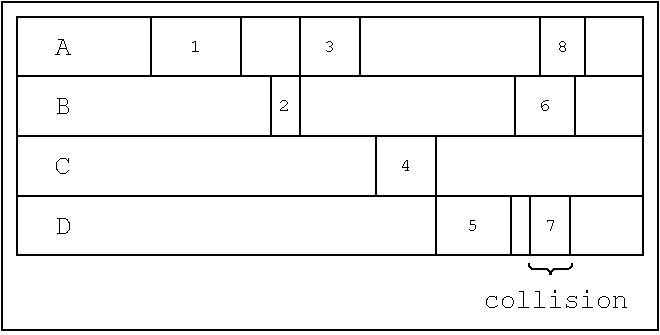
\includegraphics[width=0.8\linewidth]{images/aloha.pdf}
    \caption{An example of packets being sent by 4 stations using ALOHA.}
    \label{fig:aloha}
\end{figure}

\begin{example}[Slotted ALOHA]
    \textbf{Slotted ALOHA} is as the original ALOHA protoco; however, it introduces discrete timeslots to send packets.
\end{example}

Collisions are less common in slotted ALOHA, but still occur. The throughput compared to the standard ALOHA is significantly higher. Figure \ref{fig:slotted-aloha} illustrates the slotted ALOHA protocol.

\begin{figure}
    \centering
    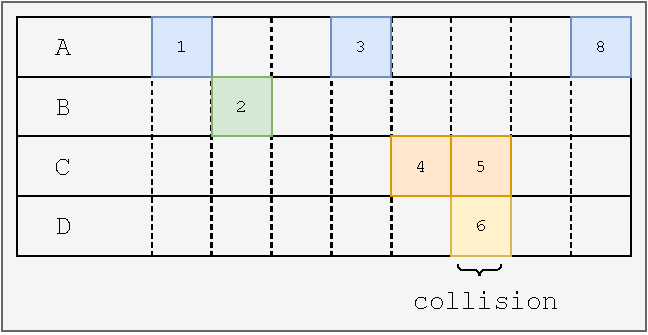
\includegraphics[width=0.8\linewidth]{images/slotted-aloha.pdf}
    \caption{An example of packets being send by 4 stations using slotted ALOHA.}
    \label{fig:slotted-aloha}
\end{figure}

\begin{definition}[Carrier sense multiple access]
    \textbf{Carrier sense multiple access} (CSMA) is a MAC protocol that checks to see if a medium is busy before transmitting data. If a medium is busy, it will not send data. 
\end{definition}

It may seem that this solves our collision problem; how can we get collisions if we never transmit when a medium is busy? Well, you may recall \emph{propagation delay} from Computer Systems I. We can not simply check if a medium is busy due to a delay in the time it takes for a data to travel down a wire.

The following are some examples of CSMA variations, so the definitions may become less rigorous (just refer to the original definitions of CSMA above).

\begin{example}[1-persistant CSMA]
    In \textbf{1-persistant CSMA}, stations continuously sense whether a medium is busy and as soon as it is it will send the frame. If there is a collision, the station will wait a \emph{random} amount of time before it resumses sensing the medium.
\end{example}

This method has a high collision chance compared to other CSMA methods (which we will see).

\begin{example}[Non-persistant CSMA]
    In \textbf{non-persistant CSMA}, if a medium is busy and a station is ready to transmit it will wait a random amount of time then it will check again. Collision handling is the same as in 1-persistant CSMA.
\end{example}

This method introduces longer delays but will reduce the chance of a collision. This is a trade-off but can improve the total throughput. 

\begin{example}[$p$-persistant CSMA]
    \textbf{$p$-persistant CSMA} works only on slotted channels. If a medium is idle, the station will transmit; however, if a medium is busy it will continuously sense the medium until it is idle then will transmit with probability $p$. If it does not transmit, it waits until the next time slow.
\end{example}

Now we can pick $p$ such that we get the best trade-off on delay with reduction in collision to get the highest throughput.

\begin{example}[CSMA collision detection]
    We can apply collision detection to CSMA by sending a \emph{jam} signal to all neighbouring stations if a collision occur. Stations should halt tranmission temporarily after receiving a jam signal.
\end{example}

Figure \ref{fig:mac-protocol-comparison} compares the different MAC protocols introduced.

\begin{figure}
    \centering
    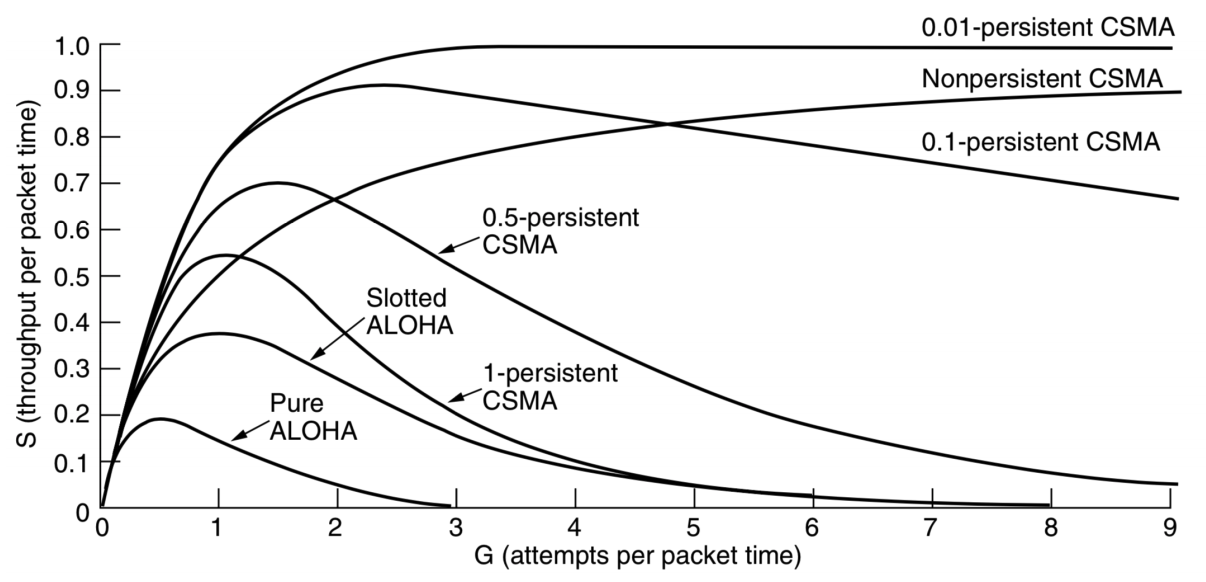
\includegraphics[width=0.8\linewidth]{images/mac-protocol-comparison.png}
    \caption{A comparison of the throughput of different MAC protocols graphed on the attempts per packet time.}
    \label{fig:mac-protocol-comparison}
\end{figure}

\begin{definition}[Controlled access protocols]
    A \textbf{controlled access protocols} is one in which each station must consult each other to see who can transmit.
\end{definition}

\begin{example}[Bitmap]
    In the \textbf{bitmap} protocol, all stations announce that they have data to transmit then they transmit in order of address (or really any decided upon order).
\end{example}

\begin{example}[Token passing]
    In \textbf{token passing}, you can only transmit data if you have a \emph{token}. Once a station has transmitted their data, they pass the token on. There can be predefined rules on how long a given station can hold onto a token for.
\end{example}

\begin{example}[Binary countdown]
    This is a relatively hard thing to explain. 
    Say that there are 4 stations that want to transmit: $A, B, C, D$. 
    Let $\operatorname{ad}{A}$ represent the address of $A$ (and similarly for the rest of the nodes). 
    Suppose these stations have $4$-bit addresses, so
    \[ \operatorname{ad}{A} = (a_1, a_2, a_3, a_4). \]
    Now we will engage in an elimination to see which station can transmit. 
    We will do this by constructing the address of the transmitting station.
    Let this address be $t = (t_1, t_2, t_3, t_4)$.
    Round 1, we calculate 
    $t_1 = a_1 \lor a_2 \lor a_3 \lor a_4$ 
    and eliminate all stations $S$ with 
    $\operatorname{ad}{S} = (s_1, s_2, s_3, s_4)$
    such that $s_1 \neq t_1$. We repeat these for the last three bits until we have one address left. 
\end{example}

\begin{example}[Example of binary countdown]
    Consider the stations with address $0010$, $0100$, $1001$, and $1010$. Then we have the following table representing the countdown.
    \begin{center}
        \begin{tabular}{ccccc}
            \toprule
            Station & & & & \\
            \midrule
            1 & 0 & 0 & 1 & 0 \\
            2 & 0 & 1 & 0 & 0 \\
            3 & 1 & 0 & 0 & 1 \\
            4 & 1 & 0 & 1 & 0 \\
            \bottomrule
        \end{tabular}
    \end{center}
    We see that $1$ and $2$ get eliminated in round 1, then no one is eliminated in round 2, then $3$ is eliminated in round 3, then (of course) no one is eliminated in round 4 giving the station $4$ the right to transmit.
\end{example}
